\documentclass[12pt,a4paper,titlepage,oneside]{scrartcl}
\newcommand{\lang}{en}
\usepackage{pp}

\usepackage{multicol}
\usepackage{amsmath, amstext, amssymb,latexsym}
\usepackage{graphicx}
\graphicspath{ {images/} }

\newcommand{\team}{2}
\newcommand{\dokumenttyp}{Report}
\newcommand{\datum}{\today}

\newcommand{\lvaname}{\ifthenelse{\equal{\lang}{de}}{Einführung paralleles
Rechnen}{Parallel Computing}} 
\newcommand{\lvanr}{184.710}
\newcommand{\semester}{WS 2016}

\newcommand{\studentAName}{Ferdinand Baarlink}
\renewcommand{\studentAMatrnr}{1635879}

\newcommand{\studentBName}{Roland Wallner}
\renewcommand{\studentBMatrnr}{1427019}


\newcommand{\colormode}{color}
%% \newcommand{\concat}{\ensuremath{+\!\!+\,}}
\newcommand{\concat}{\ensuremath{\scalebox{0.8}{++}}}
\newcommand{\merge}{\mathsf{merge}}
\newcommand{\corank}{\mathsf{corank}}


\begin{document}


%%%%%%%% TITLE PAGE %%%%%%%%%%%%%%%%%%

\begin{center}
\vspace{2.5cm}
{\LARGE\textbf \dokumenttyp\\}
\vspace{0.5cm}
{\LARGE\textbf \lvaname\\}
\vspace{0.5cm}
{\LARGE \lvanr\ -- \semester\\}
\vspace{1.0cm}
{\LARGE \datum}
\vspace{1.5cm}

{\LARGE \ifthenelse{\equal{\lang}{de}}{Gruppe}{Group} \team}
\vspace{1.5cm}

\teamnMitglieder


\end{center}

\vspace{1.5cm}

\newpage
%%%%%%%% TITLE PAGE ENDS HERE %%%%%%%%

%\setcounter{section}{0}
%\setcounter{tocdepth}{2}
\tableofcontents

\section{Introduction}
Lorem ipsum dolor sit amet, consetetur sadipscing elitr, sed diam nonumy eirmod tempor invidunt ut labore et dolore magna aliquyam erat, sed diam voluptua. At vero eos et accusam et justo duo dolores et ea rebum. Stet clita kasd gubergren, no sea takimata sanctus est Lorem ipsum dolor sit amet. Lorem ipsum dolor sit amet, consetetur sadipscing elitr, sed diam nonumy eirmod tempor invidunt ut labore et dolore magna aliquyam erat, sed diam voluptua. At vero eos et accusam et justo duo dolores et ea rebum. Stet clita kasd gubergren, no sea takimata sanctus est Lorem ipsum dolor sit amet.

\section{Solution}
For every solution we took the following approach:
The sorted input arrays $A$ and $B$ are split into parts
$A = A_1 \concat A_2 \concat \ldots \concat A_p$  and
$B = B_1 \concat B_2 \concat \ldots \concat B_p$
, in a way that all elements in $A_i \cup B_i$ are smaller then those in $A_{i+1} \cup B_{i+1}$. 
With such a distribution given, each Process $i$ merges independently $A_i$ and $B_i$ using a simple sequential merge algorithm.
Afterwards a master process concatinates the results.
The sequential merge function is in following noted by $\merge()$.

\subsection{Co-ranking}
In order to obtain a distribution as mentioned above, we implemented a co-ranking algorithm.
The idea is that for a given index $i$ of the resulting array $C$, 
the co-ranking algorithm $\corank(i)$ should yield a pair of indexes $(j,k)$
such that
\begin{equation}\label{eq:coranking1}
  C[0\ldots i-1] = \merge(A[0\ldots j-1],B[0\ldots k-1]).
\end{equation}
The impact for parallelization is the following:
Let $i$ be the id of a process,
then we make this process calculate the entries of $C[i \cdot l, \ldots, (i+1)\cdot l - 1]$,
where $l$ is the blocksize that each process calculates.
Therefore it uses the coranking algorithm to get
$(j_1,k_1) = \corank(i\cdot l)$ and $(j_2,k_2) = \corank((i+1)\cdot l)$.
With \eqref{eq:coranking1} one has
\begin{align*}
  \merge(A[j_1,\ldots,j_2],B[k_1,\ldots,k_2]) = C[i \cdot l,\ldots, (i+1)l - 1].
\end{align*}
So each process can independently both calculate the coranks and perform the merge.

To calculate the coranks we use that
$j$ and $k$, which fulfill \eqref{eq:coranking1}, are also given by the following
properties\footnote{As shown in Lemma1 in Siebert, Träff: Perfectly load-balanced, optimal, stable, parallel merge (https://arxiv.org/abs/1303.4312)}
\begin{enumerate}
  \item $j + k = i$
  \item $j = 0 \vee A[j-1] \leq B[k]$\label{first_inequal}
  \item $k = 0 \vee B[k-1] < A[j]$
\end{enumerate}
Tith leads to a binary-like search for the co-ranks.
For $j$ take an arbitrary value $\leq m$ and set $k$ so that $k + j = i$.
Also keep track of the lower limits for $j$ and $k$ in $j_{min}$ and $k_{min}$.

Now check:
If $j=0 \vee A[j-1] > B[k]$, then point 2 is violated so $j$ was too great and $k$ too small,
so set $k_{low}=k$ and try again with $j = \floor*{\middlee(j,j_{low})}$ and $k$ adjusted such that $j + k = i$.

Or if $k=0 \vee B[k-1] \geq A[j]$, then point 1 is violated and $j$ was too small.
So set $j_{low}=j$ and try again with $k = \floor*{\middlee(k,k_{low})}$ and $j$ adjusted according to point 1.

It can be proven that this infact terminates and computes the co-ranks to $i$\footnote{Proposition1 of the same source by Siebert and Träff}.

%\lstinputlisting[caption=co-ranking algorithm in C,label=code:corank,style=c]{corank.c}
%\begin{lstlisting}[caption=co-ranking algorithm in C,label=code:corank,style=c]
 % while(counter++ < (m + n)) {
  %  if( j>0  &&  k<n  &&  A[j-1]>B[k] ) {
  %    k_low = k;
  %    int diff = j-j_low, delta = diff/2 + (diff&1);
  %    j = j - delta;
  %}
%\end{lstlisting}


\subsection{Implementation}
Every implementation uses the following structure:
\begin{enumerate}
  \item read the input
  \item merge in parallel using co-ranks
  \item put the parts together
  \item check if result is ordered again
\end{enumerate}
The details for each implementation are presented in the following paragraphs.

\subsubsection{OpenMP}
In OpenMP, the programm runs sequentially in one master thread until it reaches a parallel section.
At this point new threads are created to execute this section simultaneously.
This section is marked by the directive

\textbf{\#pragma omp parallel num\_threads(p) private(a, b, ..)},

where p is the number of threads and a, b, ... are local variables.
All threads share a common address space.
If a variable is not explicitly marked as private, all threads access the same address when they use this variable.
When the parallel section is left, join ... master thread runs again.

For our implementation this means, that the master thread first reads/creates the input arrays.
Afterwards it allocates the space for the resulting array and makes it available in a public variable.
Then the parallel section is entered and the threads are created.
Each thread calculates its coranks for the indexes
$id \cdot \frac{output\_length}{number\_of\_threads}$
and
$(id+1)\cdot \frac{output\_length}{number\_of\_threads}$, where $id$ is the id of the actual thread.
Then it merges directly from the input arrays into the space that is allocated for the result.

Note here that both the output array and the input arrays are public variables for all threads.
Then the parallel segment is left and the master thread checks the result for corectness.

The following snipped shows how the parallel part


\subsubsection{Cilk}

\subsubsection{MPI}
For the MPI implementation it is assumed that the input arrays are already distributed among all processes.
In contrast to other implementation these processes need to activly communicate to calculate the coranks.
To archieve this, each process makes its array parts accessible by opening a MPI window.
This is demonstrated in \hyperref[code:mpi_window]{Listing \ref*{code:mpi_window}}.

\begin{lstlisting}[caption=window to share arrays, label=code:mpi_window,style=c]
MPI_Win_create(A, len1, sizeof(int), MPI_INFO_NULL, MPI_COMM_WORLD, &winA);
MPI_Win_create(B, len2, sizeof(int), MPI_INFO_NULL, MPI_COMM_WORLD, &winB);
\end{lstlisting}

Afterwards other processes can read from them as presented in \hyperref[code:mpi_get]{Listing \ref*{code:mpi_get}}.

\begin{lstlisting}[caption=window to share arrays, label=code:mpi_get,style=c]
int value;
MPI_Win_lock\(MPI_LOCK_SHARED, targetRank, 0, win1\);
  MPI_Get\(value, 1, MPI_INT, targetRank, d, 1, MPI_INT, win1\);
MPI_Win_unlock\(targetRank, win1\);
\end{lstlisting}

Eventually we wrote a function getValueFrom(int index,MPI\_Win win,...) for reading elements from a certain position in $A$ (or $B$).
Therefor it calculates which process has the required part of $A$ (or $B$).
If it is the same process it reads it from its own array.
Otherwise it uses the access method from \hyperref[code:mpi_get]{Listing \ref*{code:mpi_get}}.

For a MPI version of the corank algorithm, we replaced all occurrences of $A[i]$ and $B[i]$ with theValueFrom()-function.


\textbf{Problems with MPI:}
At the time of writing we had problems to run our MPI implementation with arbitrary array sizes.
So we assume that the number of processes divides the array lengths and that both arrays have the same size.
Unfortunately we could only implement a solution for INT-arrays.

\section{Testing}
We tested our solutions with different .




\section{Benchmark Setup}
For our tests we measured the time that the operation needed with the appropiate methods. So we used \textit{omp\_get\_wtime} for OpenMP, \textit{clock\_gettime} for Cilk and \textit{MPI\_Wtime} for MPI.

First we decided which problemsizes would be part of the benchmark. We agreed on the following sizes (m, n) where both input arrays will have this size:

\begin{multicols}{3}
\begin{itemize}
\item 50
\item 100
\item 1000
\item 10000
\item 100000
\item 500000
\item 1000000
\item 5000000
\item 10000000
\end{itemize}
\end{multicols}

Additionally we did tests where the first array has a different size than the second one.
\begin{center}
\begin{tabular}{l | r | r | r | r | r}
\hline
 Type & 1 & 2 & 3 & 4 \\ \hline
 m & 150000 & 50000 & 1500000 & 500000 \\ \hline
 n & 50000 & 150000 & 500000 & 1500000 \\ \hline
\end{tabular}
\end{center}

Next to the size of the arrays we needed to specify the layout of the values inside the arrays.
There is four different cases we benchmarked:

\begin{description}
\item[Interleaved] The numbers alternate between the two arrays. (e.g: array1 = \{ 1, 3, 5, 7, 9, ...\}, array2 = \{ 2, 4, 6, 8, 10, ...\})
\item[Smaller First] All numbers in the first array are smaller than the ones in the second one. (e.g: array1 = \{ 1, 2, 3, 4, 5, ...\}, array2 = \{ 10, 11, 12, 13, ...\})
\item[Smaller Last] All numbers in the first array are bigger than the ones in the second one.  (e.g: array1 = \{ 10, 11, 12, 13, ...\}, array2 = \{ 1, 2, 3, 4, 5, ...\})
\item[Random] The numbers in both arrays are still sorted, but cannot know which number is in which array. (e.g: array1 = \{ 1, 3, 4, 7, ... \}, array2 = \{2, 5, 6, 9, ... \})
\end{description}

After specifying which problemsizes and the array layouts we want to test. We specified the rest of the testing parameters. We decieded to do \textbf{35 repetitions} for each test and only use the \textbf{median time} value for further calculations.

We ran all permutations of these settings on two machines. We ran our OpenMP and Cilk together with our sequential Baseline on \textit{saturn} and a small laptop. MPI was only tested on the laptop as \textit{saturn} did not offer a working environment for MPI execution.

\begin{center}
\begin{tabular}{ l | l | l }
\hline
 & saturn & laptop \\ \hline
CPU & AMD Opteron 6168 @ 1.9GHz & Intel Core i5-5200U CPU @ 2.70 GHz \\ \hline
Cores & 48 & 4 \\ \hline
L1 Cache & 64K & 32K \\ \hline
L2 Cache & 512K & 256K \\ \hline
L3 Cache & 5118K & 3072K \\ \hline
RAM & 128 GB DDR3-1333 & 4 GB DDR3-1600 \\ \hline
\end{tabular}
\end{center}

\section{Results}


\subsection{Expected Results}



\subsection{Real Results}

\begin{figure}[h]
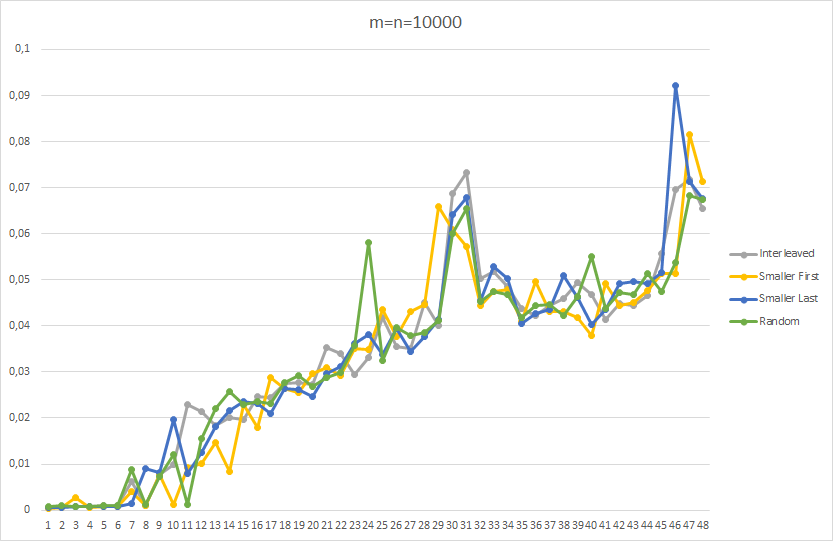
\includegraphics[width=\linewidth]{Saturn_OpenMP_10000}
\caption{OpenMP / All Modes / m=n=10000}
\label{fig:omp_allm_10000}
\end{figure}

As shown in Figure \ref{fig:omp_allm_10000} paralellization results in worse times when the sample size is too small. In this case we cannot provide enough work for each core so the more cores we add the longer the algorithm will take to merge the two arrays.

In Cilk we will see similar results. (Figure \ref{fig:cilk_allm_10000}) But here we can see an improvment at the start. When looking at the graph we can conclude that if you have a problem size of m=n=10000 it is more efficient to use Cilk with 6 to 7 workerthreads than using only one or more than 10.

\begin{figure}[h]
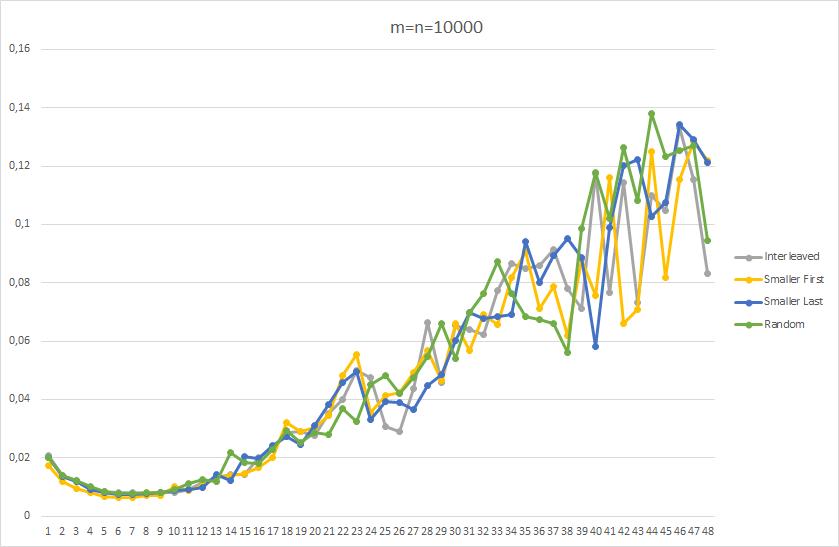
\includegraphics[width=\linewidth, height=0.6\linewidth]{Saturn_Cilk_10000}
\caption{Cilk / All Modes / m=n=10000}
\label{fig:cilk_allm_10000}
\end{figure}
\begin{figure}[h]
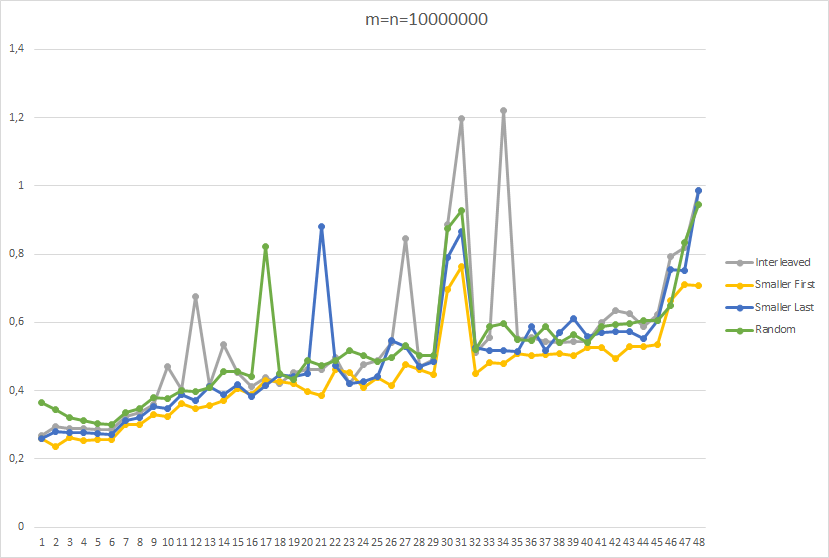
\includegraphics[width=\linewidth, height=0.6\linewidth]{Saturn_OpenMP_10000000}
\caption{OpenMP / All Modes / m=n=1000000}
\label{fig:omp_allm_10000000}
\end{figure}

When the problemsize gets bigger we can see a similar curve with OpenMP. (Figure \ref{fig:omp_allm_10000000}) Here  we can see that the paralell algorithm sped up the calculation until 6 cores if you have random values. After that, more cores mean more time. Another interesting bump in Figure \ref{fig:omp_allm_10000000} is that all different modes take longer if 30 or 31 cores are used. We think that this is related to problematic cache sceduling, but we did not investigate any further.

\begin{figure}[h]
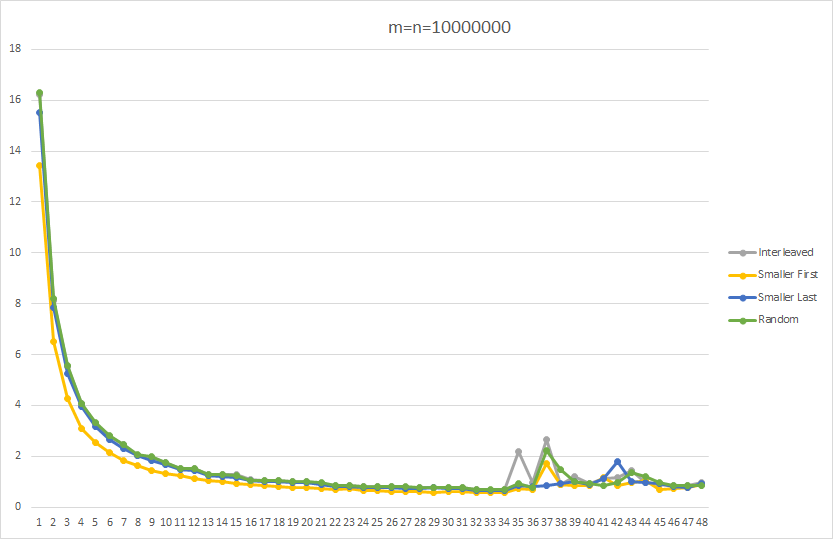
\includegraphics[width=\linewidth]{Saturn_Cilk_10000000}
\caption{Cilk / All Modes / m=n=10000000}
\label{fig:cilk_allm_10000000}
\end{figure}

For \textit{cilk} we can see very interesting behaviour. The algorithm is really slow when using few cores. This is caused by the fixed amount of tasks that are created for \textit{cilk}. We are always creating 48 packets. This results in a huge sceduling overhead as the work sceduler has to switch between packets more often than it should be needed.

\begin{figure}[h]
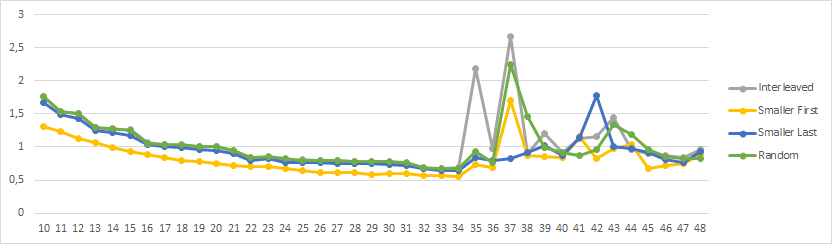
\includegraphics[width=\linewidth]{Saturn_Cilk_10000000_Cut}
\caption{Cilk / All Modes / m=n=10000000 / p > 9}
\label{fig:cilk_allm_10000000_cut}
\end{figure}

If you remove the first few cores (Figure \ref{fig:cilk_allm_10000000_cut}) you can see that the algorithm scales really well and still gets faster when 34 cores are used.
This seems to be really good, but looks less pleasing if you compare the results to the times of our \textit{OpenMP} solution. (Figure \ref{fig:comparison_cilk_omp_random_10000000}) Cilk is still very slow in comparison.

\begin{figure}[h]
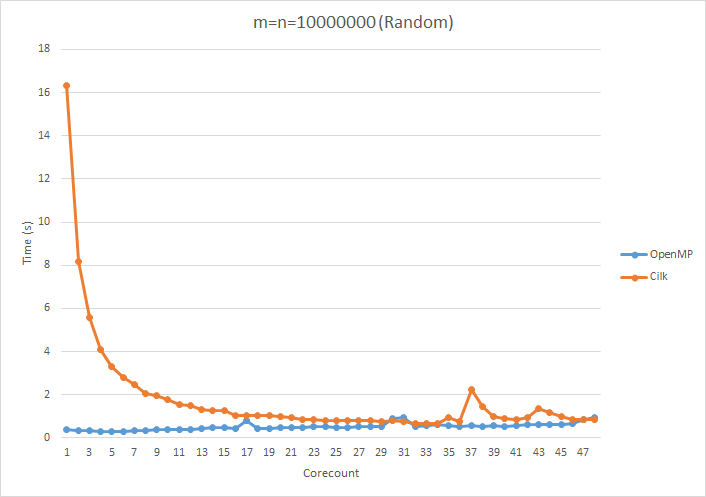
\includegraphics[width=\linewidth]{Saturn_Random_10000000}
\caption{Comparison: OpenMP/Cilk}
\label{fig:comparison_cilk_omp_random_10000000}
\end{figure}

Even though our paralell algorithms are slow for the problem sizes we tested, the trends seems to be that they work for bigger problemsizes. We managed to produce a small speed-up for p=7, m=n=10000000. (Figure \ref{fig:saturn_omp_speedup_random}) The speedup can be observed when looking at our random mode, as there is worse branch-prediction of the processor, which can be taken out of the calculation then. It seems that branch-prediction did increase the speed of our sequential solution so our paralell algorithms could not reach it easily.

\begin{figure}[h]
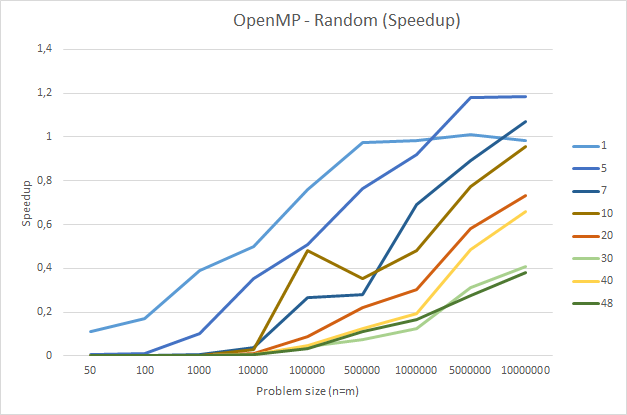
\includegraphics[width=\linewidth]{Saturn_OpenMP_Speedup_Random}
\caption{OpenMP Speedup}
\label{fig:saturn_omp_speedup_random}
\end{figure}

Either way, we were not able to reach any positive speedup in our \textit{cilk}-implementation. (Figure \ref{fig:saturn_cilk_speedup_random})

\begin{figure}[h]
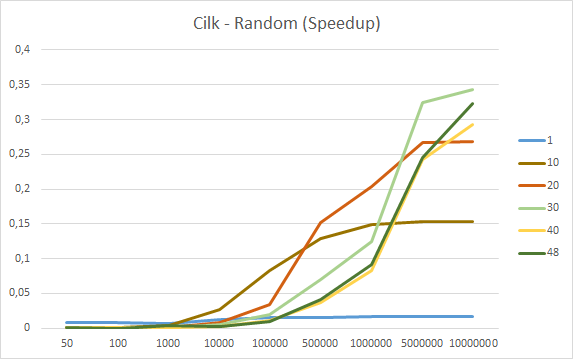
\includegraphics[width=\linewidth]{Saturn_Cilk_Speedup_Random}
\caption{Cilk Speedup}
\label{fig:saturn_cilk_speedup_random}
\end{figure}

\section{Summary}


\section{Beispiele}
\subsection{Source Code formatieren}
Es folgen einige Beispiele wie Sourcecode in diesem Dokument formatiert und referenziert werden kann
(\hyperref[code:beispiel1]{siehe Listing~\ref*{code:beispiel1} auf Seite~\pageref*{code:beispiel1}} und \hyperref[code:beispiel2]{siehe Listing~\ref*{code:beispiel2} auf Seite~\pageref*{code:beispiel2}}).

Ebenso können kurzer Code oder kurze Befehle direkt in der Zeile in einem \lstinline{lstinline Block} mit typengleicher Schrift formatiert werden.

\lstinputlisting[caption=Example C/C++ file,label=code:beispiel1,style=c]{corank.c}

\begin{lstlisting}[caption=Example bash script,label=code:beispiel2,style=simple]
#!/bin/bash
echo "Bash version ${BASH_VERSION}..."
for i in {0..10..2}
  do
     echo "Welcome $i times"
 done

echo "some very very very very very very very very very very very very very very very very very very very very long string"

exit 0;
\end{lstlisting}

\subsection{Bilder}

Es folgen einige Beispiele wie Bilder in diesem Dokument eingefuegt werden koennen
%(\hyperref[fig:cilk01]{siehe Abbildung~\ref*{fig:cilk01} auf
%Seite~\pageref*{fig:cilk01}}).

%\begin{figure}[h!]
  %\centering
  %\fbox{
    %\includegraphics[width=0.8\textwidth]{./imgs/graph1.png} %width in prozent.
  %}
  %\caption{Cilk: n = 1 000 000}
  %\label{fig:cilk01}
%\end{figure}


%%%%%%%%%%%%%%%%%%%%%%%%%%%%%%%%%%%%%%%%%%%%%%%%%%%%%%%%%%%%%%%%%%%%%%
%
% DO NOT CHANGE THE FOLLOWING PART
%
%%%%%%%%%%%%%%%%%%%%%%%%%%%%%%%%%%%%%%%%%%%%%%%%%%%%%%%%%%%%%%%%%%%%%%

\end{document}


